\begin{center}
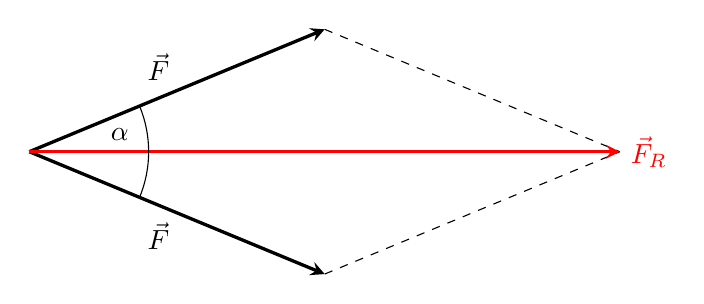
\begin{tikzpicture}[>=stealth]
 \draw[->, very thick] (0,0) -- (3.751,1.554);
 \node[above left] at (1.9,0.78) {$\vec F$};
 \draw[->, very thick] (0,0) -- (3.751,-1.554);
 \node[below left] at (1.9,-0.78) {$\vec F$};
 \draw[dashed] (3.751,1.554) -- (7.5,0);
 \draw[dashed] (3.751,-1.554) -- (7.5,0);
 \draw[->, very thick, red] (0,0) -- (7.5,0) node[right] {$\vec F_\text{R}$};
 \draw (1.4,-0.58) arc (-22.5:22.5:1.515);
 \node at (1.15,0.22) {$\alpha$};
\end{tikzpicture}
\end{center}

Das Kräfteparallelogramm zweier gleich grosser Kräfte ist ein Rhombus. Die Diagonale $\vec F_\text{R}$ halbiert den Winkel $\alpha$ und steht senkrecht auf der anderen Diagonalen. Jede Kraft trägt deshalb $F\cos(\alpha/2)$ zur Resultierenden bei:
\begin{align}
 F_\text{R} &= 2\,F\cos\frac{\alpha}{2}
\end{align}
Aufgelöst nach $F$:
\begin{align}
 F &= \FGlF \\
   &= \frac{\FRg}{2\cdot\cos\left(\alGO/2\right)} \\
   &= \FGl \approx \result{\FGlP{0}{2}}
\end{align}
